\documentclass[violet]{main}
\begin{document}
	\maketitle
	\makeflypage
	\frontmatter
	\tableofcontents
	\mainmatter
	\Fancy
	\chapter{执行概要}
		\section{公司概述}
			南京洛克斯科技有限责任公司是一家拟成立的科技公司,致力于外卖员配送外卖到小区与顾客取走外卖之间的临时存储。产品拥有完全自主知识产权 ,软硬件相结合,完美解决了外卖配送最后一百米的困难。公司秉承提高服务效率、增强安全性能的愿景,减小外卖配送员送货及顾客取走外卖的安全隐患,节约双方时间,并保证了外卖食品的存储的卫生与新鲜。
		\section{项目概述}
			本团队打造的智能外卖储存柜具备远程智能温控保存和空气循环系统,满足消费者对餐品的温度要求解决了气味残留问题。外卖柜的信息传输基于微信小程序,配送员在同一设备启动配送界面,小程序便可自动读取配送信息,当餐品入柜后自动发送验证码到订餐者手机,节省了在柜前输入手机号的时间,更方便对接''美团''、''饿了么''等外卖平台,更容易普及投入使用。
		\section{市场分析}
		\section{竞争分析}
		\section{人事分析}
		\section{财务分析}
		\section{风险分析}
	\chapter{公司概述}
		\section{公司简介}
			\subsubsection{公司名称}
				南京洛克斯科技有限责任公司,洛克斯来自英语Lockers的音译,意为食品储存柜或寄物柜,直接阐明了公司的产品类型。
			\subsubsection{公司产品}
				“Lockers”智能外卖自助存取柜
			\subsubsection{公司标志}
				\begin{center}
					\Tcbset\tcbox[title = \hypertarget{公司标志}{公司标志}]{\includegraphics[width = 7cm]{logo.eps}}
				\end{center}
			\subsubsection{公司理念}
				勇于改变,争创一流!
				\\\indent 诚信为本,客户至上!
			\subsubsection{公司使命}
				让订餐者享受更优的外卖配送服务!
			\subsubsection{公司文化}
				秉承“勇于改变,争创一流”的发展理念,努力开展团队建设,不断拓宽客户渠道;
				\\\indent “以竞争促团结,以团结促发展”,公司鼓励各部门之间开展良性竞争,以竞争促使团队更加和谐、团结,以和谐、团结的队伍奠定公司的发展基础;
				\\\indent “责任在心,服务至上”是公司的营销理念,公司本着对客户负责任的态度提供产品,并用用无微不至的服务打动客户,发展客户。
		\section{公司选址}
			综合对公司市场分布地区的考察比较,我们将办公地址选定在南京理工大学国家大学科技园,主要基于如下考虑:
			\begin{strength0}{\it 优势明显的平台公司——南京理工科技园股份有限公司}{}
				\it 平台公司本身具有很强的造血功能和投资管理功能,是平台公司中少有的“高新技术企业”。这不仅能为园区企业孵化、大学生创业提供必要的经济支撑,同时也是园区管理人才的实战平台。
			\end{strength0}
			\begin{strength0}{\it 现代高效的运行体制}{}
				\it 南理工科技园是典型的校府合作模式,是定位于企业化运营管理的大学科技园。
			\end{strength0}
			\begin{strength0}{\it “四园合一”、“三区联动”的区位优势}{}
				\it 校园、创新园、服务园、产业园 ——“四园合一”
				\par 校区、园区、社区 ——“三区联动”
				\par 毗邻高速、高铁—— “交通便利
			\end{strength0}
		\section{商业模式}
			\subsection{市场定位}
				公司的市场定位一方面是高校、写字楼和一些小区的外卖消费者,另一方面是外卖的递送员。
			\subsection{产品定位}
				能为配送员提高配送效率,保护订餐者隐私的智能外卖自助存取柜
			\subsection{商业目的}
				解决当今外卖派送车泛滥照成的安全问题、提升外卖派送效率、保护订餐者详细住址隐私,给消费者更优的外卖体验。
			\subsection{核心优势}
				经过调研发现,当今外卖市场存在很多问题,配送员为了赶速度、拼业绩,无视交通法规;
				\\\indent 部分人群不能在外卖送达的第一时间取餐,尤其是在校园内,外卖被误取、冒的现象频频发生;用餐高峰期,外卖派送时间普遍增长,难以在预期时间取到外卖;外卖配送员骚扰客户,产生纠纷的事件增多,消费者家庭住址等隐私被侵犯。
				\\\indent 在这样的行业背景之下,公司的产品--Locker应运而生。
				\\\indent Lockers 智能外卖存取柜,从配送员到达指定小区至Lockers发送出取餐短信只需要30秒,首创使用语音输入订餐者信息,大大提高存柜效率。在用餐高峰期,当同一个小区有多位客户时,Lockers的效率优势更加显著。Lockers还为消费者提供了外卖寄存的场所,就算延迟下班也能顺利取到美食,同时它保护了消费者的隐私,不暴露门牌号等信息,避免了配送员与订餐者的直接接触,减少了发生冲突的可能。
			\subsection{经营模式}
				“Lockers”柜子的服务对象是外卖订餐者和外卖骑手。一般放在人口集中区的居民楼、宿舍、写字楼等不方便派送的地区。作为派送员和消费者的中间媒介,派送员到达目的,自动验证身份即可语音或手动输入订餐者信息,将外卖入柜,并实时向消费者发送验证短信,消费者收到短信后自行前往领取外卖。
			\subsection{盈利模式}
				公司将充分发挥大学生创业的优势,积极利用员工的专业资源,通过推销校内各大宿舍小区购买,慢慢形成的品牌效应,逐渐推向其他高校组织公司盈利来源主要由以下几个方面:1、通过为骑手提高效率,收取骑手存柜费用2、为订餐者提供外卖寄存的场所,向订餐者收取寄存费用3、在外卖储存柜上设广告位,收取广告商家费的广告宣传费用。
		\section{发展战略}
			\subsection{初期战略}
				目前,公司的第一版产品“Lockers”智能外卖存取柜的生产方案已经初步完成,得到了南京理工大学电子工程与光电技术学院同学和老师的大力支持,目前正在积极与南京理工大学其他组织社团、其他各大高校联系,进行产品的推广和功能升级。在公司成立之初,力求以高质量的产品和热情周到的服务迅速打入市场,形成自己的品牌效应,立足于外卖配送柜领域。
				\begin{description}
					\item[市场策略]根据公司市场发展规划,在第一年,着重针对于以南京为中心的江苏省地区,主要面向江苏省内特别是南京地区的知名高校学院院办楼以及学生宿舍小区。
					\item[销售策略]主要采用直接营销的策略,通过有针对性的对于特定高校进行上门推销,利用技术先进性和价格优势,开辟属于公司的智能外卖存取柜市场,并利用现有的成熟产品对新市场实现渗透,打造公司在外卖配送柜领域的领导领先地位。
					\item[研发策略]在开拓市场的同时,注重收集整理客户对产品的反馈和建议,做好客户意见调查,并实时了解客户的最新需求,对产品进行改进和优化。
				\end{description}
				\subsection{中期战略}
					中期,在调整产品的同时,进一步拓展新市场,提高市场占有率。并注重外卖储存柜的功能开发技术学习投资,保持先进的技术,使公司的产品能够不断的更新,跟上需求的发展,并维持公司良好的信誉和知名度。
				\begin{description}
					\item[市场策略]开拓江苏省内市场的同时,进一步调整产品,并积极拓展江苏地区以外的华东地区的高校宿舍以及学院院办楼、居民住宅楼。江苏省内特别是南京地区的写字楼、中小型公司,扩大销售市场,进一步提高市场占有率。
					\item[销售策略]对于江苏省内市场,由于目标客户供求的特殊性,公司仍应主要采取直接销售的模式,各大高校、公司直接联系,上门推销。通过初创期的市场开拓,公司在业界已经形成了一定的知名度,合理利用已有的口碑来扩大销售,在科学的市场调研下继续积极主动的拓宽目标市场,建立新的客户关系。
					\item[研发策略]针对产品的各个指标,如收货短信的发送,语音输入的功能完善,储存柜的开锁安全等功能进行改进和完善,使产品的优势更加突出。
				\end{description}
			\subsection{长期战略}
				后期,公司注重技术投资,保持技术领先;注重技术人才计划的实施,储备优秀人才。
				\begin{description}
					\item[市场策略]在稳固华东市场的同时,积极拓展除华东市场外的教育发达的大省,例如广东省、北京市、湖北省、河南省、天津市等。公司发展后期,在稳定华东地区市场后,将仍然有重点的针对以上非华东地区的 5 大省份进行市场拓展。在成熟期,更应注重市场的稳定和产品的功能更新、缺陷的优化,以先进的技术和优秀的人才作为公司的核心竞争力,将公司发展壮大。稳固在华东市场的高校、中小型公司的同时,继续积极拓展浙江省、北京市、湖北省、天津市、四川省、重庆市、河南省、上海市八大省市的市场。另一方面,可以考虑整合市场资源,与同类的外卖存取柜商家达成战略联盟,为客户提供列更功能更加完善齐全的外卖储存柜。
					\item[销售策略]由于市场规模进一步扩大,公司将继续巩固与国内的知名外卖存取柜商家的产品代理合作,拓展中部,东部外卖市场。
					\item[研发策略]由于外卖存取柜发展时间较短,功能、技术还不够完善,外卖平台,市场功能更新快,要及时进行市场的调研和分析,针对市场需求的不同变化,采取不同的措施,进行不同方面的技术学习培训投资。
				\end{description}
		\section{组织形式}
			\subsection{组织结构}
				\begin{center}
					\Tcbset\tcbox[title = \hypertarget{组织结构}{组织结构}]{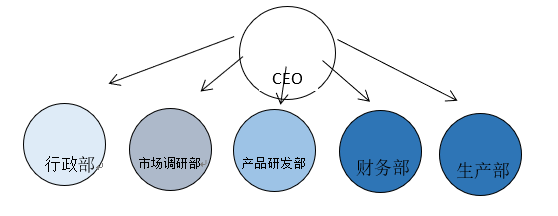
\includegraphics[width = 7cm]{graph3.png}}
				\end{center}
				在公司创业初期,由于生产规模较小、目标市场较为集中,发展战略中心在市场的开拓以及技术的革新,组织结构拟采用简洁明了的直线式管理结构。由首席执行官对四个部门直接进行管理,高度集中的简单线性结构、精简的组织层次有利于管理者对公司人员集中控制,提高决策效率,缩减公司的管理运营成本。
			\subsection{部门职责}
				根据公司运营需要,在 首席执行官下设置四个部门,各部门的职责如下:
				\begin{description}
					\item[首席执行官]主要负责统筹公司工作,直接管理四个部门,制定公司方针路线,并负责与外界公司以及相关部门沟通。
					\item[行政部]主要负责公司内部事务的管理协调。其一,负责公司的行政事务,具体化战略目标,协调优化各个部门之间的关系和沟通,并与政府部门对接。其二,制定人力资源规划,并实时按照战略目标规划调整优化人力资源的招聘、培训、绩效等计划,并协调各部门人力资源的分配。其三,管理公司的财务会计工作,负责公司资金的筹集、使用和分配,确定公司的资本结构以及投资决策,制定财务计划及财务预、决算,并负责各期财务报表,及时对公司财务投资做出分析,及时对财务风险提出预警。
					\item[调研部]主要负责公司的市场调研、营销推广和客户关系管理。第一,需要对公司目标市场进行详细的调查研究,抓住目标客户群体;第二,采取积极的营销策略和措施,以拓展市场和扩大销售;第三,负责公司客户关系维护,基于服务行业的标准,为客户提供优质的售前、售后服务,维护好与客户的关系和沟通交流,及时获取客户的反馈评价。
					\item[研发部]主要负责公司产品核心技术的研发和改进,并与生产部共同负责产品的生产工作。依托本团队的人才优势,在不断完善和改进现有产品和技术的基础上进行下一步的研发,积极主动的抓住市场的需求,开发新的产品,有效决断的拓展新的应用领域。在生产环节中,研发部根据客户需求开展设计工作,提供给生产部生产所需的设计方案;并对零部件、组装过程中的两大模块及最终的成型产品的质量进行严格的检验,确保产品质量符合出厂要求;同时,根据客户的使用反馈,重新改进设计。
					\item[财务部]负责公司日常财务核算,参与公司的经营管理。根据公司资金运作情况,合理调配资金,确保公司资金正常运转。严格财务管理,加强财务监督,督促财务人员严格执行各项财务制度和财经纪律。负责全公司各项财产的登记、核对、抽查的调拨,按规定计算折旧费用,保证资产的资金来源等。
					\item[生产部]主要负责在研发部协作下进行公司产品的生产管理。首先,根据市营部提供的订单信息和研发部提供的设计部安排生产;其次,根据产品生产所需的原材料进行零部件的采购,并协调与供应商的合作关系;而后,对产品进行组装与调试。另外,生产部还将负责售后服务中的产品及技术的维护。
				\end{description}
			\subsection{部门关系}
				首席执行官负责统筹全局,直接管理四个部门。
				\begin{description}
					\item[行政部]负责各部门之间的协调和沟通,对各部门工作成效进行考核;负责人力资源的招聘和分配,以及员工的考核和绩效;发放各部门的资金预算。
					\item[研发部]加强与售后部的沟通交流,及时优化产品功能;对市营部的销售人员进行必要的技术、专业知识的培训,以更好地与需求客户进行沟通交流,促进销售。
					\item[调研部]获取技术部最新的技术研发进程,以利于在与客户沟通时加强其对公司核心技术的信心;在产品售后的维护中,及时与生产部沟通和交接;整理汇总客户资料,交于客服部进行定期客户关系维护和信息分析。为技术部提供客户反馈以进一步优化和改进产品;对市营部的客户及时提供优质的服务。
					\item[财务部]搜集公司经营活动情况、资金动态、营业收入和费用开支的资料并进行分析、提出建议,定期向总经理报告。组织各部门编制收支计划,编制公司的月、季、年度营业计划和财务计划,定期对执行情况进行检查分析。
					\item[生产部]及时向技术部反馈生产中的问题,尽快解决以维护公司产品的高质量;从市营部中及时获取客户的反馈,进一步优化生产;对客服部的客户关系服务提供必要的产品维护。
				\end{description}
		\section{创业团队}
			\subsection{管理团队}
				\begin{wrapfigure}{l}{4cm}
					\Tcbset\tcbox[title = \hypertarget{首席执行官——鄢军勇}{首席执行官——鄢军勇}]{
\includegraphics[width = 3.5cm]{YanJunyong.jpg}}
				\end{wrapfigure}
				\hyperlink{首席执行官——鄢军勇}{首席执行官——鄢军勇}
				介绍:就读于电子工程与光电技术学院,光电信息科学与工程专业。曾任南京理工大学电光学院年级团学联宣传部部长,现任9161040G06班班长负责班级常规事务,曾获得电光学院2016级“最赞班长称号”,“科技活动积极分子称号”。预备党员,大学期间成绩良好,多次获得奖学金。
				\begin{wrapfigure}{r}{4cm}
					\Tcbset\tcbox[title = \hypertarget{财务总监——顾鑫想}{财务总监——顾鑫想}]{
\includegraphics[width = 3.5cm]{GuXinxiang.jpg}}
				\end{wrapfigure}
				\hyperlink{财务总监——顾鑫想}{财务总监——顾鑫想}
				介绍:南京理工大学2016级会计学本科生,掌握财务方面知识,系统学习了公司税务财务方面的基础。现任职创业中心助理,了解大学生创业相关事宜。参与过ERP沙盘模拟课程培训,对企业营运过程较为熟悉。
				\begin{wrapfigure}{l}{9cm}
					\Tcbset\tcbox[title = \hypertarget{营销总监——黄海群}{营销总监——黄海群}]{
\includegraphics[width = 3.5cm]{Huanghaiqun.jpg}}
				\end{wrapfigure}
				\hyperlink{营销总监——黄海群}{营销总监——黄海群}
				介绍:会计学本科生,在校成绩优异,曾数次获得奖学金,掌握一定的财务知识和市场营销技能。现任校社团南理工英语俱乐部副社长,擅长与人沟通交流,负责举办多次大型活动并担任主持人。参加ERP沙盘模拟大赛并获得校赛二等奖,对公司的实际运营有所了解。
				\begin{wrapfigure}{r}{4cm}
					\Tcbset\tcbox[title = \hypertarget{产品总监——吴振宇}{产品总监——吴振宇}]{
\includegraphics[width = 3.5cm]{WuZhenyu.jpg}}
				\end{wrapfigure}
				\hyperlink{产品总监——吴振宇}{产品总监——吴振宇}
				介绍:
				\begin{wrapfigure}{l}{4cm}
					\Tcbset\tcbox[title = \hypertarget{市场总监——周康虎}{市场总监——周康虎}]{\includegraphics[width = 3.5cm]{Zhoukanghu.jpg}}
				\end{wrapfigure}
				\hyperlink{市场总监——周康虎}{市场总监——周康虎}
				介绍:在大一学年,担任年级团学联副主席一职,发挥自己的语言和组织能力,组织并且参加了各类综合活动。在学院双旦晚会、多米诺骨牌比赛中担任主持人;2017年暑假参加学院薪火党员工作站组织的暑期社会实践,荣获江苏省“三下乡”社会实践优秀团队、江苏省优秀调研报告。平时关注时事政治,积极参加社会实践和志愿服务,并于2017年12月9日成为年纪首批预备党员。大学期间成绩不断进步,排名位于年级前15\%,获得奖学金。现今在薪火党员工作站担任活动部部长一职,充分发挥主观能动性,组织参与了一批高质量的活动。
				
						\section{管理团队}
						\section{创业团队}
						\section{人力资源}
							\subsection{员工招聘}
							\begin{center}
								\Tcbset\tcbox[title = \hypertarget{员工招聘}{员工招聘}]{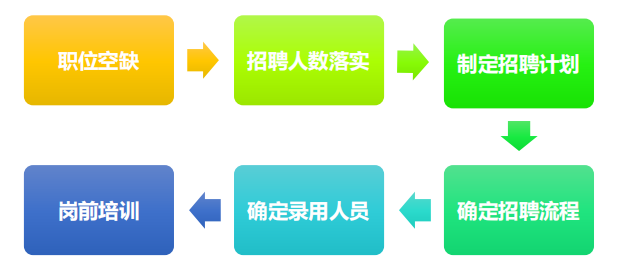
\includegraphics[width = 7cm]{graph4.png}}
							\end{center}
								公司成立第一年,我们重点招聘高级专业技术人才和高级管理人才,同时招募各部门员工。
								公司成立初期,主要通过外部招募的方式来吸引人才。我们将通过员工推荐、职业介绍机构等方式吸纳人才。
								各部门根据公司未来发展战略规划确定职位空缺,提出《人力资源需求申请表》。行政部总负责员工的招聘,根据各部门的人才需求,落实招聘人数。并编制招聘计划,通过人才市场、网络工具、校园招聘等渠道联络人才,并安排各部门所需人员的面试。面试合格的人员,在试用 6个月,满足各项要求后正式录用,并办理各项录用手续。人事专员需将新员工的身份证复印件存入《备用人才》文件夹,应聘资料录入电脑,为该员工按照工号编号规则拟定工号并办理考勤卡一张。安排新员工体检,出现异常的,及时提请行政部处理。
			\subsection{员工培训}
				在公司内部,我们建立专业培训师资网络,对所聘可授课人员进行资格认证;在公司外部,我们将与相关大学、培训机构、咨询公司建立起外部培训网络。根据公司自身特点,有针对性地开发培训项目,对公司及外部人员进行培训。
				\begin{description}
					\item[公司员工]我们就公司文化、知识技能、工作态度等方面对其进行系统性培训。通过有计划、有组织的培训,提高员工素质,增强员工归属感,从而增强企业的竞争力。对于招聘的新员工,除对其进行系统培训外,还将从中选择一定数量的表现出众者,对其进行特殊培训,作为公司发展的后备军。在培训过程中,公司将注重对员能力的挖掘,提升员工能力,规划员工发展方向。
					\item[基层人员]我们对其着重进行管理培训、行为培训,在提升其管理能力的同时,加强其基层操作能力、熟悉基层作业流程,做到身体力行,知与行齐头并进。临时性员工培训:公司将对其进行简单的技能培训、行为培训,提高人员素质,保证产品质量。
				\end{description}
			\subsection{员工薪酬}
				公司制定基本工资时,参考了南京市人社局发布的 2017 年企业在岗职工工资指导价格,拟定工资标准如下表所示。公司在不同时期制定了不同的工资标准,为了更好地稳定公司的组织架构,控制员工流失率,激励公司上下共同进步,公司计划从第二年开始,按照每年 10\%的增长率,增加员工基础工资。此外随着业务发展、规模扩大,也会增加员工人数。公司根据南京市社保管理中心和住房公积金管理中心的有关规定,以员工工资为参照,设计员工社保和公积金的计算基数,为员工提供良好的福利待遇,更好地激励公司员工积极工作。详见下表。
				\begin{center}
					\Tcbset\tcbox[title = \hypertarget{法人单位与产业活动单位在各省、自治区、直辖市的分布情况}{法人单位与产业活动单位在各省、自治区、直辖市的分布情况}]
					{	\arrayrulecolor{blue!50!black}\renewcommand{\arraystretch}{1.2}
						\begin{tabular}{c|c|c|c|c}
							部门					&	职位			&	人数		&	人均月薪酬/元·	&	合计/元	\\\hline
							首席执行官			&	首席执行官	&	1		&	9350				&	112200	\\\hline
							\multirow{2}*{研发部}	&	经理			&	1		&	7810				&	93720	\\\cline{2-5}
												&	职员			&	3		&	7040				&	84480	\\\hline
							\multirow{2}*{财务部}	&	经理			&	1		&	7480				&	89760	\\\cline{2-5}
												&	职员			&	3		&	5830				&	209880	\\\hline
							\multirow{2}*{调研部}	&	经理			&	1		&	6490				&	77880	\\\cline{2-5}
												&	职员			&	3		&	5940				&	213800	\\\hline
							\multirow{2}*{生产部}	&	经理			&	1		&	5720				&	68640	\\\cline{2-5}
												&	职员			&	6		&	5170				&	372240	\\
						\end{tabular}
					}
				\end{center}
		\paragraph{工资说明}
			\begin{description}
				\item[基本工资]企业员工的固定报酬,均为月薪制。
				\item[激励工资]工资中随着员工工作努力程度和劳动成果的变化而变化的部分,如随着员工工作努力程度变化而变化的工资,随着员工劳动产出的变化而变化的工资。例如:销售人员通过自身努力达到规定的销售目标,帮助公司提升产品销量,这些均将作为绩效考评的内容之一,来确认激励工资。
				\item[特殊奖金]对员工超额劳动的报酬,如全勤奖金、生产奖金、不休假奖金、年终奖金、效益奖金等。
				\item[津贴补贴]对员工在工作环境中的额外劳动消耗和生活费用的额外支出的补偿。如岗位津贴、加班津贴、轮班津贴
			\end{description}
	\chapter{项目概述}
		\section{项目背景}
			当下,随着移动互联网行业的迅速发展,移动互联网餐饮外卖服务倍受消费者的青睐。互联网餐饮外卖是指以互联网为媒介,通过网站、APP应用等途径进行线上订餐。它打破了传统电话外卖的方式,借助互联网这个巨大的信息平台,以外卖资源整合为核心,以消费者需求为导向,也为消费者提供庞大的外卖信息以及方便的送餐服务,使消费者足不出户就可以享受到美味、健康、快捷的外卖美食。同时,为餐饮从业者提供了新的销售和宣传渠道,能够在已有的营业额基础上实现规模的巨大扩张,也满足了广大消费者新的需求。移动互联网的快速发展、智能手机和电子信息技术的成熟、大学生群体、白领群体等其他年轻消费者的作息时间特殊性,带动了互联网餐饮外卖行业的飞速发展,前景可观。
			\\\indent 当下的外卖行业具有餐饮外卖消费群体广阔、方便快捷、价格实惠等特点:
			\begin{strength}{\it 消费群体(尤其是年轻群体)庞大}{}
				\it 从团队在南京理工大学的调查分析来看,有过使用网络平台订餐经历的学生已占大学生群体的85%以上。由此可见,外卖平台在年轻群体的普及率极高,在年轻群体中,使用外卖平台订餐已经成为一种常见的饮食消费方式。
			\end{strength}
			\begin{strength}{\it 方便快捷}{}
				\it 与电话点餐等传统外卖方式不同,外卖020平台打破了传统的外卖单订餐方式,用户使用外卖020平台点餐的操作更简单,更方便快捷。在消费者的体验焦度,用户不需要掌握各家外卖的联系方式及菜单等具体信息,只需要打开外卖平台的软件,进行餐品点选,最终付款。平台方作为商户和消费者的中间方,会代替用户完成通知商户、下单等具体细节操作,并向用户提供订单处理的流程。因此,方便快捷将成为它继续发展的主要优势,并且也将是它与传统商业竞争的重要优势。
			\end{strength}
			\begin{strength}{\it 技术支持强大}{}
				\it 当下主打的外卖订餐app有“美团外卖”“饿了么”“滴滴外卖”等,其背后的公司都具备着雄厚的经济和技术支持,能够顺应市场需求,调整服务范围和类型。例如,美团外卖推出了“生鲜果蔬”、“送药上门”购的服务,解决了白领上班早没时间买菜和一些特殊人群没时间买药的问题。
			\end{strength}
			但是,外卖行业的发展也存在着一些问题:
			\begin{weakness}{\it 交通安全问题}{}
				\it 网络订餐为市民的生活带来了不少便利,但为了赶速度、拼业绩,随之而来的交通违法行为屡见不鲜,安全隐患频现对于很多外卖小哥而言,闯红灯、逆行等早已成为家常便饭,他们自信不会出什么事情然而,其他市民对此却是深恶痛绝不少市民表示,这些事件无论对于机动车驾驶员、行人还是外卖小哥自身,都会带来极大的危害。
			\end{weakness}
			\begin{weakness}{\it 信用体系不完善}{}
				\it 消费者在利用外卖020平台订购餐饮时,对于提供商品的商户方的具体信息并不了解。在餐品配送过程中,外卖配送人员与消费者之间也是陌生人与陌生人的关系。近年来,随着外卖配送、快递配送行业的发展,一些关于配送员与订餐者之间的矛盾纠纷屡见不鲜。派送员作为一个陌生人却知道消费者的联系电话和家庭住址,并有机会让消费者为陌生人开门验收外卖。近年来被派送人员骚扰与派送人员发生口角冲突的事件层出不穷。
			\end{weakness}
			在这样的行业背景之下,公司的产品---Lockers应运而生。本产品着眼当下外卖市场的发展痛点,致力于:
			\begin{center}
				\begin{tcolorbox}[title = {发展目标}]
					为外卖消费者带来更安全舒适的订餐服务;
					\tcblower
					为派送员节省更多的派送时间提高派送效率。
				\end{tcolorbox}
			\end{center}
		\section{产品组成}
			公司的产品---Lockers由\hyperlink{外卖柜箱体}{外卖柜箱体}和\hyperlink{人工操作模块}{人工操作模块}两部分组成。
			\begin{center}
				\Tcbset\tcbox[title = \hypertarget{外卖柜箱体}{外卖柜箱体}]{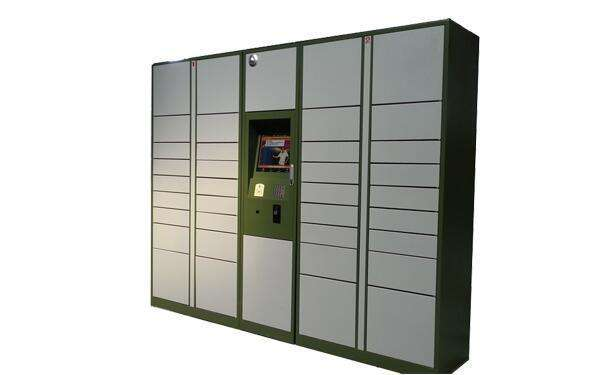
\includegraphics[width = 7cm]{cabinet.jpg}}
			\end{center}
			\begin{center}
				\Tcbset\tcbox[title = \hypertarget{人工操作模块}{人工操作模块}]
				{	\arrayrulecolor{blue!50!black}\renewcommand{\arraystretch}{1.2}
					\begin{tabular}{c|c}
						显示屏广告区	&	机械键盘输入区	\\\hline
						触屏操作区	&	语音输入区		\\
					\end{tabular}
				}
			\end{center}
		\section{技术介绍}
			自助外卖存取柜主要包括一台PC设备、智能电控锁模块、紫外线杀菌模块、语音输入系统和监控摄像头等模块。
			\begin{center}
				\Mindmap
			\end{center}
			\begin{center}
				\Flowchart
			\end{center}
		\section{产品特点}
			近年来,外卖行业发展迅速,但仍然存在着日益突出的几大问题:
			\begin{enumerate}
				\item 外卖配送员为了赶速度、拼业绩,无视交通法规,违法行为屡见不鲜,带来了巨大的交通安全隐患。
				\item 多数学生和白领群体由于工作性质,不能在外卖送达的第一时间取餐,尤其是在校园内,外卖被误取、冒领等丢失的现象时有发生。
				\item 用餐高峰期,外卖派送时间普遍增长,用户难以在预期时间取到外卖。
				\item 外卖员骚扰客户,与客户产生纠纷的事件增多,客户家庭住址等隐私被侵犯。
			\end{enumerate}
			\par Lockers 智能外卖存取柜,从配送员到达指定小区至Lockers发送出取餐短信只需要30秒,在用餐高峰期,当同一个小区有多位客户时,Lockers的效率优势更加显著。Lockers还为消费者提供了外卖寄存的场所,就算延迟下班也能顺利取到美食,同时它保护了消费者的隐私,不暴露门牌号等信息,避免了配送员与订餐者的直接接触,减少了发生冲突的可能。
		\section{产品优势}
			\begin{enumerate}
				\item 首创语音输入结合自助存取柜,大大提高了派送员的送餐效率,平均每份外卖存柜时间只需15秒,在用餐高峰期也能保证订餐者准时收到餐品。
				\item 配备紫外线杀菌灯,保证食品储存环境内的卫生安全,提升订餐者的消费体验。
				\item 避免了派送员在骑行过程中打电话,同时极大的节约了外卖派送的人力资源,缓解了由于派送员电动车泛滥造成的交通拥堵问题,消除了骑行过程中打电话、闯红灯等现象带来的安全隐患。
				\item 在柜子的上端有一个小型视频监控器,详细记录取物与寄物的人的外貌特征。可以为意外发生的丢失物品等小概率事件提供寻找的证据,大大提高安全系数。
				\item 全天24小时服务,无论何时订餐,都能够前来提取餐品。
			\end{enumerate}
		\section{代际更迭}
		\section{权威认证}
		\section{质量鉴定}
		\section{服务概述}
		\section{发展规划}
	\chapter{市场分析}
		美团点评研究院发布的\href{http://b2b.toocle.com/detail--6431901.html}{《2017年中国外卖发展研究报告》}显示,2017年在线外卖市场规模突破2000亿元,同比增长23\%;在线订餐用户规模达3亿人,同比增长18\%。随着生活质量的逐步提升,外卖不仅提供送餐服务,更可以满足消费者生活方方面面的需求。同时报告显示,用户的外卖选择正在从单一的餐饮品类扩展到全品类,其中生鲜果蔬、甜点饮品、生活超市等类目的订单量正在快速增长,增长率均高于200\%。本公司主打的“Lockers”智能外卖储存柜在食品质量保障和食材保鲜上有技术的支持和市场竞争优势,在外卖柜这一萌芽行业具有市场核心竞争力。
		\section{PEST分析}
			\subsubsection{政治因素}
				中国第一部专门针对快递业的行政法规\href{http://www.xinhuanet.com/politics/2018-03/27/c\_1122599567.htm}{《快递暂行条例》}自 2018年5月1日起施行,国家就快递行业的健康发展表现出重视和监管的必要性。外卖服务在一定程度上与快递服务存在着共通之处,尤其是他们面临的信息泄露问题。因此在国家鼓励最后一公里配送多样化,优化末端派件的智能共享设施背景下,智能外卖柜、快递柜应运而生,能够为消费者提供优质服务。两会热议的食品安全问题,不仅需要从源头抓起,督促商家提供优质食品,保障外卖骑手自身卫生情况,还需要坚持末端派送的食品保鲜保温,为消费者提供温度适宜、口感绝佳的餐饮食品。
			\subsubsection{经济因素}
				随着共享经济时代的到来,快递快送业务高速增长。移动互联网、大数据技术的不断发展,互联网浪潮不断影响传统餐饮企业,“互联网+餐饮”已覆盖半成品餐饮、餐饮企业服务管理、网络订餐和互动分享全流程服务。艾瑞数据显示,2015年我国餐饮外卖市场规模已超过2300亿,占整体餐饮消费的比例为7.4\%,到2018年,这一比例有望达到14.8\%,外卖市场整体规模也将超过6600亿,如\hyperlink{2010-2018年中国餐饮外卖市场规模及占餐饮行业比重}{2010-2018年中国餐饮外卖市场规模及占餐饮行业比重}所示。在生活节奏加快以及我国政府提出扩大内需的背景下,外出就餐和外卖送餐将逐渐成为我国越来越多用户的餐饮消费习惯,餐饮外卖市场的交易规模也将保持较高的增长速度。
				\begin{center}
					\Tcbset\tcbox[title = \hypertarget{2010-2018年中国餐饮外卖市场规模及占餐饮行业比重}{2010-2018年中国餐饮外卖市场规模及占餐饮行业比重}]{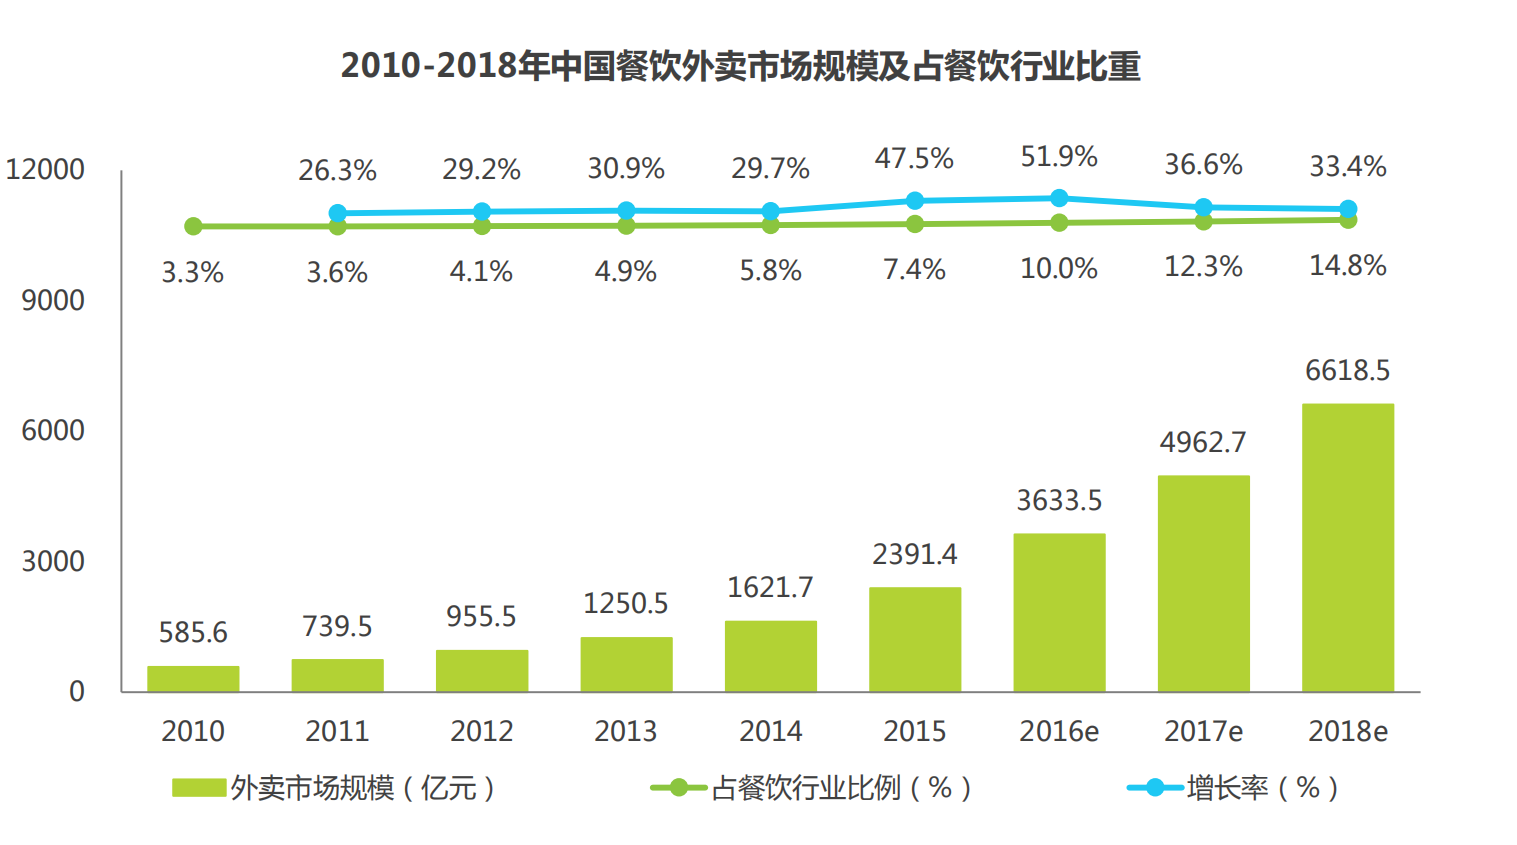
\includegraphics[width = 10cm]{graph.png}}
				\end{center}
				\par GDP的增长,居民人均可支配收入的提升以及“懒人经济”都为外卖O2O的发展提供了机遇,如\hyperlink{2010-2018年城镇居民人均可支配收入及增长率}{2010-2018年城镇居民人均可支配收入及增长率}所示。此外,外卖O2O作为新业态在支撑就业方面发挥了重要作用。目前外卖是最被看好的O2O发展领域之一,巨额融资为其快速发展提供了良好的资金基础。
				\begin{center}
					\Tcbset\tcbox[title = \hypertarget{2010-2018年城镇居民人均可支配收入及增长率}{2010-2018年城镇居民人均可支配收入及增长率}]{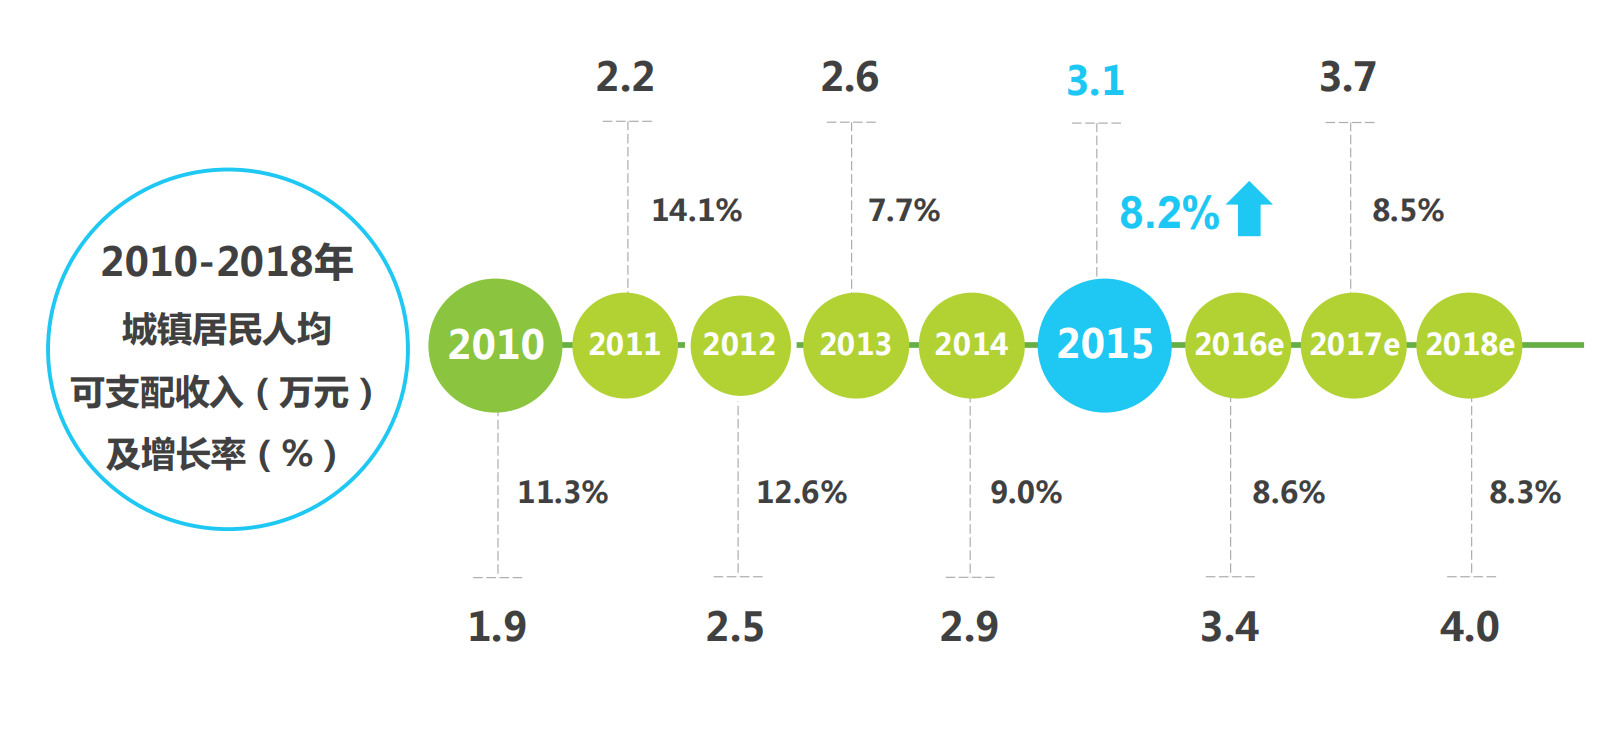
\includegraphics[width = 10cm]{graph2.png}}
				\end{center}
				\par 在互联网+、移动支付、懒宅经济及平台博弈等的大趋势推动下,外卖未来的发展空间前景无限,有待提升和进步的地方也需要着重关注。外卖行业不能因为速度而怠慢了服务,不能因为速度而忽视了安全。
			\subsubsection{社会因素}
				外卖行业的兴起促进了就业以及餐饮服务行业线下至线上的革新,同时造成了许多安全问题。首先,外卖行业的薪酬模式给外卖员业务过程中带来了很大的安全风险。送餐车在非机动车道上如脱缰野马到处乱窜、横冲直撞,有时还一边看手机一边骑车,想转弯的时候就转弯,不遵守交通规则的现象屡见不鲜,让人提心吊胆。分析其中的原因,是收入随单量阶梯浮动的薪酬模式促成了业务员这种多拉快跑的现场。外卖骑手的种种不良表现,给城市交通安全以及自身的安全都造成了极大的不良影响。
				\\\indent 与此同时,顾客订单中信息的泄露,包括电话号码、顾客被外卖员电话骚扰,乃至接收外卖时发生的肢体接触,都给消费者不良的客户体验,同时对快递骑手这一工作引起的危机不可谓为不大。外卖员的身份问题难以确认以及保障业主的住宅安全,很多公寓都禁止外卖员进入小区,与业主产生直接接触,因此最后一公里的上门配送是外卖行业很大的挑战,对外卖员的业务量以及送餐效率提升造成了很大的阻碍。
			\subsubsection{技术因素}
				根据CNNIC第41次\href{http://www.cac.gov.cn/2018-01/31/c\_1122347026.htm}{《中国互联网络发展状况统计报告》},截止2017年12月,中国网民规模达7.72亿,互联网普及率为55.8\%,互联网惠及全民取得新进展,互联网商业模式不断创新,线上线下服务融合加速,信息化服务快速普及;截止2017年12月,我国手机网民规模达7.53亿,网民中使用手机上网占比达97.5\%,移动网络促进“万物互联”,移动互联网服务场景不断丰富,移动终端规模快速提升,为移动互联网产业创造更多价值空间。
				\\\indent 移动端设备的普及与移动技术的发展推动消费场景多元化,互联网得以渗透居民生活的每个角落,服务范围向更深更广阔扩散。越来越多的消费者习惯通过手机来满足日常生活中的各类需求,餐饮行业的线上化已是大势所趋。随着80、90后伴随着互联网成长起来的一代逐渐成为消费主力,消费者对于便捷性、个性化和品牌化要求进一步提升,对餐饮行业精细化、数据化运营能力的要求越来越高。互联网浪潮的冲击下,餐饮行业的互联网化飞速发展。从最初的点评模式开始,团购、外卖等诸多模式不断涌现,当前,餐饮行业已成为本地生活服务行业中互联网化程度最高的行业之一,订外卖、在线预订、团购都已经成为消费者就餐的常规选择。
		\section{行业分析}
			随着外卖行业的快速发展,外卖员与消费者的对接主要是送货上门、当面确认,鲜少有第三方只能自助媒介统一收取外卖,提供收货、保管、提货的便捷高效服务。当今市场的储存柜主要有”丰巢”快递柜和”乐栈”保险柜,前者只提供快递寄存服务,不能满足餐品的保温和杀菌,后者则需要使用乐栈专用的app才能将餐品配送到柜,由于餐品种类少而不能普及。快递柜行业仍处于萌芽阶段,竞争并不激烈,同时由于快递柜是刚刚开始发展的行业,在这一阶段中,购买者对产品尚未熟悉,企业无法实现规模经济导致高价格、分销渠道发展不完善。
			\\\indent 在行业发展初期,本公司将面临着在生产、采购、销售等方面成本较高,缺乏学习和经验效应的劣势;在这一阶段,行业的进入壁垒来自掌握技术上的诀窍而不是规模经济所要求地成本或品牌忠诚,因此现有企业将受到保护。如何更有效地教育顾客、打开分销市场、完善产品设计将成为本企业发展初期的战略导向。
			\subsubsection{目标市场}
				公司产品主要应用于外卖服务的末端派件,同时能够提供保温消毒灯附加功能,为消费者提供优质的外卖体验和服务。根据公司战略规划,公司发展初期目标市场主要为江苏省各大高校以及居民楼、事业单位等办公场所;随着产品研发的不断成熟、市场竞争越发激烈,公司发展中期会将市场扩展到华东地区的高校以及办公场所、居民住宅,获取规模效应带来的成本控制优势;之后在行业技术的发展与支持,更多的竞争者将加入到市场角逐中,公司最终将充分挖掘全国市场对外卖柜的需求,进一步扩展市场份额。
			\subsubsection{市场描述}
				\paragraph{全国高校}
					根据教育部官方网站最新发布2017年全国高等学校名单,截至2017年5月31日,全国高等学校共计2914所,普通高等学校2631所(含独立学院265所),成人高等学校283所,其中江苏省高校数量占首位。
					\\\indent 随着 O2O 商业模式的快速发展,诸如“饿了么”“淘点点(口碑外卖)”“百度外卖”“美团外卖”等越来越多的网上外卖订餐平台涌现。以大学生为对象的 O2O 外卖订餐行业蓬勃发展。因此大学生往往是订购外卖的主力军之一,江苏省高校数量一定程度上代表了外卖订单数量以及外卖骑手进出校园频次。考虑到江苏省高校的潜在需求量极大,公司第一步发展战略应当定位在对校园安全以及食品安全监管力度大的高校内,尤其是江苏省高校。
				\paragraph{办公场所}
					根据国家统计局统计结果,分省、自治区、直辖市看,2001年末,拥有法人单位数名列全国前10位的依次是:广东、江苏、浙江、山东、河南、四川、上海、北京、河北、辽宁,占全国的58.4\%。拥有产业活动单位数名列全国前10位的依次是:广东、山东、江苏、浙江、河南、四川、上海、河北、湖南、安徽,占全国的55.1\%。江苏省法人单位个产业活动单位在全国来看一直都名列前茅。江苏省近些年经济发展与技术创新和新技术接受度也比较高。因此公司初步应当集中资源开拓江苏市场。如\hyperlink{法人单位与产业活动单位在各省、自治区、直辖市的分布情况}{法人单位与产业活动单位在各省、自治区、直辖市的分布情况}和\hyperlink{江苏省各地区基本状况与个体工商业发展情况对照表}{江苏省各地区基本状况与个体工商业发展情况对照表}所示:
					\begin{center}
						\Tcbset\tcbox[title = \hypertarget{法人单位与产业活动单位在各省、自治区、直辖市的分布情况}{法人单位与产业活动单位在各省、自治区、直辖市的分布情况}]
						{	\arrayrulecolor{blue!50!black}\renewcommand{\arraystretch}{1.2}
							\begin{tabular}{c|c|c}
										&	法人单位/万	&	产业活动单位/万	\\\hline
								全国		&	510.7			&	708.8				\\
								北京 	&	24.7 			&	26.6				\\
								天津		&	9.3			&	10.2				\\
								河北		&	21.9			&	29.4				\\
								山西		&	12.6			&	21.0				\\
								内蒙古	&	7.3			&	10.9				\\
								辽宁		&	21.8			&	27.6				\\
								吉林		&	8.7			&	11.7				\\
								黑龙江	&	10.8			&	17.5				\\
								上海		&	25.9			&	33.6				\\
								江苏		&	40.2			&	48.2				\\
								浙江		&	36.0			&	43.1				\\
								安徽		&	17.9			&	28.4				\\
								福建		&	15.7			&	23.2				\\
								江西		&	14.7			&	21.3				\\
								山东		&	34.9			&	50.4				\\
								河南		&	26.8			&	37.5				\\
								湖北		&	16.2			&	25.3				\\
								湖南		&	18.8			&	29.1				\\
								广东		&	40.3			&	53.5				\\
								广西		&	12.3			&	18.9				\\
								海南		&	3.1			&	4.3				\\
								重庆		&	9.0			&	14.2				\\
								四川		&	26.0			&	37.1				\\
								贵州		&	8.6			&	12.7				\\
								云南		&	9.8			&	16.5				\\
								西藏		&	1.6			&	2.2				\\
								陕西		&	16.3			&	22.7				\\
								甘肃		&	8.3			&	13.8				\\
								青海		&	2.1			&	3.0				\\
								宁夏		&	2.5			&	3.4				\\
								新疆		&	6.6			&	11.5				
							\end{tabular}
						}
					\end{center}
					\begin{center}
						\Tcbset\tcbox[title = \hypertarget{江苏省各地区基本状况与个体工商业发展情况对照表}{江苏省各地区基本状况与个体工商业发展情况对照表}]
						{	\arrayrulecolor{blue!50!black}\renewcommand{\arraystretch}{1.2}
							\begin{tabular}{c|c|c|c}
										&	地区人口/万	&	各地GDP/亿元 &	个体工商户/人	\\\hline
								全省 	&	7304.36		& 	9511.91		&	1648008		\\
								南京		& 	612.62		&	1150.30		&	148497		\\
								无锡		& 	508.66		&	1360.11		&	110856		\\
								徐州 	&	891.40		&	715.71		&	145501		\\
								常州 	& 	377.63		&	672.9			&	123408		\\
								苏州 	& 	679.22		&	1760.28		&	194837		\\
								南通 	& 	751.29		&	809.30		&	194468		\\
								连云港 	&	456.99		&	315.82		&	72905		\\
								淮安 	& 	503.82		&	329.02		&	98122		\\
								盐城 	& 	794.65		&	603.23		&	150679		\\
								扬州 	& 	458.86		&	505.46		&	113384		\\
								镇江 	& 	284.49		&	502.66		&	84404		\\
								泰州 	& 	478.58		&	449.97		&	134943		\\
								宿迁 	& 	506.16		&	223.16		&	76004		
							\end{tabular}
						}
					\end{center}
					\par 根据江苏省第二次全国基本单位普查有关数据,该普查将私营企业分为私营独资企业、私营合伙企业、私营有限公司、股份有限公司四类,全省共有各类私营企业155234家。江苏省企业数量庞杂,大型企业员工福利较好,用餐问题一般都能在员工食堂得到解决,因此私营的中型企业更符合公司市场定位,其平均从业人数与外卖柜的存储容量也较为匹配。如\hyperlink{江苏私营企业基本情况表}{江苏私营企业基本情况表}所示:
					\begin{center}
						\Tcbset\tcbox[title = \hypertarget{江苏私营企业基本情况表}{江苏私营企业基本情况表}]
						{	\arrayrulecolor{blue!50!black}\renewcommand{\arraystretch}{1.2}
							\begin{tabular}{c|c|c|c}
								类型			&	企业个数	&	百分比/\%&	平均从业人数	\\\hline
								私营独资		&	78533	&	50.59		&	19.99			\\
								私营合伙		&	9811		&	6.32		&	26.76			\\
								私营有限		&	62268	&	40.11		&	30.10			\\
								私营股份有限	&	4622		&	2.98		&	36.70			\\
								总计			&	155234	&	100.00	&				
							\end{tabular}
						}
					\end{center}
		\subsubsection{销量预测}
			由于本公司处于初期创业阶段,产品知名度和市场影响不高,因此在公司战略规划初期,公司将立足于江苏省重点高校,因此第一年销量72台;随着市场不断扩大,规模效应作用的发挥,第二年将达到144台销量;第三年、第四年本产品将投入到华东地区进行市场营销,市场范围进一步扩大,销量随之也将达到可观数量;第五年本公司将打开全国市场上品牌知名度,挖掘更多个性化、多样化产品需求。
			\begin{center}
				\Tcbset\tcbox[title = \hypertarget{销量预测}{销量预测}]
				{	\arrayrulecolor{blue!50!black}\renewcommand{\arraystretch}{1.2}
					\begin{tabular}{c|c|c|c|c|c}
						年份			&	1	&	2	&	3 	&	4	&	5	\\\hline
						销量预测/台	&	72	&	144	&	288	&	576	&	1152
					\end{tabular}
				}
			\end{center}
		\subsection{波特五力}
			由宏观环境分析可知,整体宏观环境对外卖柜的发展非常有利。但是外卖柜行业内也面临着激烈的竞争和技术不成熟造成的市场扩张压力。行业内的竞争环境,决定公司与产品能否在行业内立足并获得超额利润。公司利用竞争五力分析模型,从五个方面识别并分析行业内竞争力量对公司产品的影响。
			\subsubsection{买方影响}
				买方对行业的影响主要取决于买方与行业的讨价还价能力。由于现今外卖送货上门服务的便利性往往使人忽视了信息泄露、人身安全等重大问题,因此对外卖柜的潜在市场需求量还有待挖掘,一开始消费者对外卖柜的价格敏感度较高,产品不能通过高价打开市场,而是利用技术带来的便利性和产品的不断研发打开市场销路;但是,本产品首创的语音输入结合自助存取柜,配备紫外线杀菌灯,能够保证食品储存环境内的卫生安全,提升订餐者的消费体验,与目前市场上的同类产品相比在技术上有创新和成本投入,具有较大差异,涉及开发成本较高,与此同时市场期初产品将以竞争导向辅以低价渗透的方式定价,因此买方议价能力不高。
			\subsubsection{供方影响}
				本产品主要由人工操作模块和外卖柜箱体构成。软件部分的核心技术本公司尚未掌握,因此在成本花费上价格较高,对供方市场的价格变动议价能力较低;硬件部分的技术含量较低,市场上形成了统一的定价,因此价格影响较小。具体情况可参照买方对行业的影响。
			\subsubsection{替代威胁}
				替代品给行业产品的价格制定了一个上限。由于外卖柜的普及度不高,市面上大多的外卖柜还没有实现本产品首创的紫外线杀菌、语音输入、保温等增值效果,因此本产品定价无市面产品可以参照,同时替代品成本较低所带来的定价低于本产品的价格问题,应当纳入产品定价的考虑因素中,防止替代品低价策略抢夺市场份额。
			\subsubsection{潜在威胁}
				当外卖柜市场具有较高投资回报率时,势必吸引很多潜在加入者参与到竞争中。本产品的开发仍处于萌芽阶段,在产品生产初期潜在加入者的威胁较小,随着市场不断扩大,逐渐形成行业内的企业规模效应,以及通过不断的技术创新打开高端服务的用户市场,形成老顾客对“Lockers”智能存储柜品牌的独特认识和忠诚度,潜在加入者的威胁将大大缩小对本公司的影响。
			\subsubsection{行业竞争}
				目前外卖柜行业内企业数量较少,其中做得比较好的“丰巢”、“乐栈”在目标市场和细分市场与本产品之间竞争不大,行业比较稳定,给企业创业初期提供了较大的发展空间。
				\begin{center}
					\Tcbset
					\tcbox[title = \hypertarget{行业竞争}{行业竞争}]
					{	\arrayrulecolor{blue!50!black}\renewcommand{\arraystretch}{1.2}
						\begin{tabular}{c|c|c|c}
									&Lockers智能外卖自助存储柜							&丰巢																												&乐栈
							\\\hline
							服务		&提供外卖储存服务,以及紫外线杀菌						&提供快递行业最后一公里方案服务																						&享受智能、品质、安全的预订餐饮服务
							\\\hline
							操作		&语音输入结合自助存取柜,平均每份外卖存柜时间只需15秒	&寄件:关注丰巢微信公众号,绑定手机号,选择我要下单,按照指示进行操作寄件取件微信公众号或支付宝服务窗扫码取件或者输码取件	&通过网站、app预约下单,即可在线下使用智能取餐柜自助取餐
							\\\hline
							功能		&配备紫外线杀菌灯,上端有一个小型视频监控器,广告位展示	&支持多家快递公司在线下单的寄递服务并规范电子运单统一管理,满足消费者寄件、取件双重需求									&具有0-60℃智能温控、安全消毒杀菌、逾期报警、多屏广告位展示等功能
						\end{tabular}
					}
				\end{center}
		\section{CROT分析}
			由上述分析可得,公司所处外部环境整体乐观,但仅仅拥有良好的外部环境与竞争优势不能给公司带来高额的利润。公司应拥有不可复制的核心技术并结合自身能力来利用外部环境提供的机遇。资源能力的结合对机遇的利用与威胁的规避有基础地位,而外部环境与内部资源能力的整合,对公司战略的制定产生影响。
			\\\indent CROT 矩阵分析就是结合公司外部环境以及内部资源能力进行分析,并根据外部环境机遇威胁的大小与能力资源的强弱定位公司战略。
			\\\indent 以下是公司根据外部环境及内部能力强弱,形成公司战略定位的 CROT(能力—资源—机会—威胁)分析矩阵,针对矩阵四种情况,将公司发展战略定位于扩张战略。
			\subsubsection{能力因素}
				企业有意在未来的市场上获取巨大的利润份额,就必须建立起能对未来顾客所重视的价值起巨大作用的核心竞争力。本公司的核心竞争力是优于市场上其他外卖柜的技术投入以及低价策略。同时公司将不断研究消费者需求,开发新技术和新产品,以顾客为导向多样化、个性化投放智能存储柜。
				\\\indent 公司将发挥扁平化企业组织结构带来的创新能力和组织能力,努力构建学习型组织,随着形式不断变化,具有进化和应变能力。组织素质是一个组织的根本优势所在,本公司将不断培养和修炼组织素质,发挥美味员工的专业性和团队的集成力量,提高企业持续增长的内在动力。
			\subsubsection{资源因素}
				企业的资源包括有形资源和无形资源。公司将通过前期积累增强对财务资源、物质资源、人力资源、组织资源的调动能力,发挥公司产品质量信誉的竞争优势,不断开发技术资源和创新资源,形成品牌效应和消费者对产品质量、可靠性、优质便捷服务的认知,与多家供应商形成有效率和效力的互相支持的互惠互利合作关系。
			\subsubsection{机会因素}
				在外卖行业蓬勃发展的市场条件下,外卖骑手的人数每天以井喷式的速度增长,外卖送单人员良莠不齐,给消费者造成极大的安全隐患;同时,快递骑手面临的交通安全问题、最后一公里配送困难问题,都有待解决。随着共享经济在各个行业渗透,外卖行业也急需共享设备,解决以上问题,减少外卖员与消费者直接接触以及消费者信息被外卖员随意掌握。尤其是考虑到难以进入的高校和住宅区,可以发现外卖柜的潜在需求量很大。同时,两会热议的食品安全问题,不仅需要从源头抓起,督促商家提供优质食品,保障外卖骑手自身卫生情况,,还需要坚持末端派送的食品保鲜保温,为消费者提供温度适宜、口感绝佳的餐饮食品。
			\subsubsection{威胁因素}
				外卖柜行业仍处于萌芽阶段,消费者对新事物接受度可能不高,同时消费者可能需要花费时间去熟悉外卖存储柜使用流程的操作。在形成消费者对产品可靠性以及感知易用性的过程中,市场反应的好坏将威胁到公司管理的可持续发展能力。同时在外卖柜上应用的技术优势不能成为公司后续发展的竞争优势,导致替代品较多,随着市场不断成熟,新的加入者将加剧市场竞争、缩减利润空间,使得公司盈利能力下降。
				\\\indent 根据宏观环境及内部资源能力的分析结果,对公司的\hyperlink{CROT战略分析定位矩阵}{CROT战略分析定位矩阵}进行分析,结果显示公司有足够资源和能力抓住外部机遇。树立以“战略资源——重要机遇——核心能力”的战略定位逻辑,确定公司的战略为扩张战略。公司扩张战略的表现形式是公司产品推广地域的扩大、员工团队的扩大、固定资产的增加、延伸产品的推广等等。
				\begin{center}
					\Tcbset\tcbox[title = \hypertarget{CROT战略分析定位矩阵}{CROT战略分析定位矩阵}]{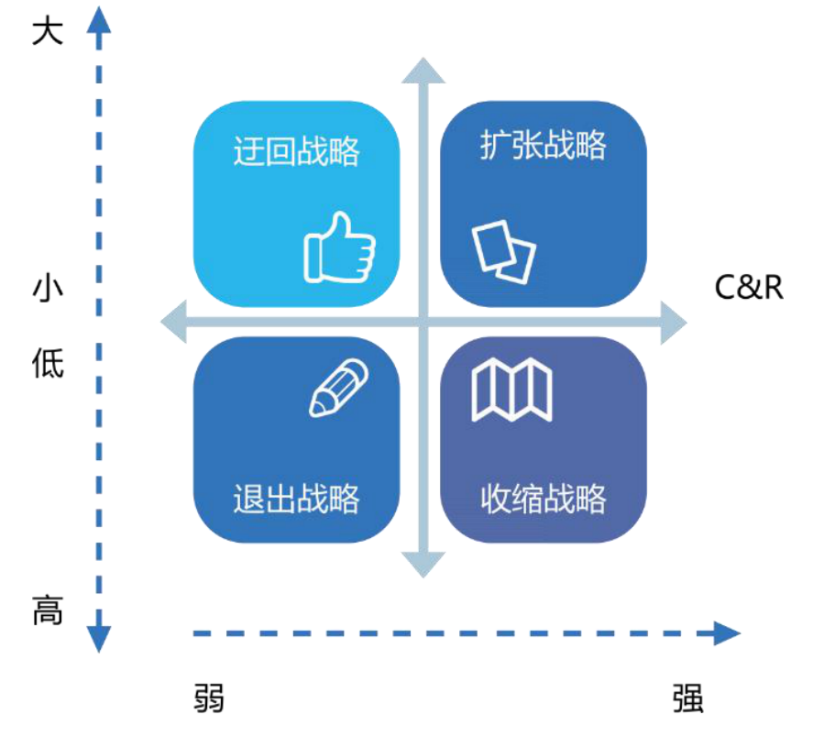
\includegraphics[width = 10cm]{graph5.png}}
				\end{center}
			根据宏观环境及内部资源能力的分析结果,对公司的 CROT 战略矩阵进行分析,结果显示公司有足够资源和能力抓住外部机遇。树立以“战略资源——重要机遇——核心能力”的战略定位逻辑,确定公司的战略为扩张战略。公司扩张战略的表现形式是公司产品推广地域的扩大、员工团队的扩大、固定资产的增加、延伸产品的推广等等。
		\section{SWOT}
		\section{市场现状}
			随着外卖行业的成熟,如今外卖派送车越来越多,给校园交通带来了很大问题,经过团队调查察发现,用餐高峰期,派送员在等待顾客拿外卖上话费很多时间,导致他们不得不加速或各种违规驾驶(例如边开车边打电话)节省时间送下一家 带来了安全隐患。
			\\\indent 另外,很多学生和上班族倾向于在下班前一段时间下单外卖,一旦派送员没有如期送至,则会导致外卖无处寄存甚至被冒领的情况。产品概述产品定位先进性成熟度核心竞争力价格低在线与便携效率高。
		\section{市场前景}
		\section{目标市场}
		\section{营销策略}
		\section{商业模式}
		\section{政策导向}
		\section{细分市场}
		\section{市场差异}
		\section{市场预测}
			\subsection{市场容量}
			\subsection{市场销量}
		\section{市场预测}
		\section{市场环境}
		\section{领域细分}	
	\chapter{竞争分析}
		\section{竞争优势}
		\section{对手分析}
			当今市场的储存柜主要有丰巢快递柜和乐栈保鲜柜,前者只提供快递寄存服务,不能满足餐品的保温和杀菌,后者则需要使用乐栈专用的app才能将餐品配送到柜,由于餐品种类少而不能普及。
			\subsection{丰巢快递}
			\subsection{乐栈保鲜}
	\chapter{运营分析}
		\section{战略选择}
		\section{商业模式}
			我们的柜式外卖寄存恒温柜主要是通过将骑手送来的外卖放入恒温柜子中,然后外卖寄存恒温柜发送短信的方式通知购买外卖的消费者,柜子的服务对象是订购外卖的消费者和各大外卖平台的外卖骑手。
			\\\indent 柜子一般放在人口集中区的居民褛、写字褛等地区的一褛,骑手到达目的地后通过扫描二維胃卜卖放入柜中,柜子实时向消费者发送外卖送达的短信,消费者收到短信后自行前往恒温柜领取外卖,每单柜子向骑手或者外卖平台收取0.5元至1元不等的服务费。
			\\\indent 在提升效率方面,外卖寄存恒温柜主要是减少了外卖骑手的等待消费者时间,提升了效率,而消费者也不会因为外卖骑手过早打电话而提前下楼浪费时间。
			\\\indent 另外在人身安全方面,因为外卖寄存恒温柜自动向消费者发送短信,不需要外卖骑手打电话通知消费者,完全避免了外卖骑手在路上因为打电话而形成的安全隐患,大大减少了送餐过程中的风险,而且避免了消费者和骑手的直接见面,也减少了可能出现的人事冲突,减少两者之间的摩檫产生。
		\section{生产组织}
		\section{质量控制}
		\section{组织管理}
		\section{人事管理}
			\subsection{服务营销}
	\chapter{营销分析}
		公司成立初期以江苏省内的 985、211 重点高校中外卖不能送到宿舍的学生或者老师、大型写字楼中的工作者、部分小区的住户为目标客户,首先和美团外卖、饿了吗和百度外卖取得一些合作,再采用直销与代理销售相结合的方式,利用产品、价格和渠道等多策略推广产品。公司将通过销售人员提供产品试用、广告宣传以及与渠道伙伴联合开展营销活动等方式开展促销活动。此外,公司还将持续为目标客户和外卖骑手提供完善的系统服务,覆盖售前、售中及售后全过程,实时监控消费者的外卖在路上的情况,努力提高客户对产品的满意度,外卖骑手对于产品的认可度,逐渐建立公司的品牌效应。
		\section{营销方案制定}
			\subsection{营销思路}
				公司在切入和渗透市场的过程中,面临着目标客户对新生的,前沿性的新型产品的接受时间长,接受程度低的困难。公司的主要产品为Lockers智能外卖储存柜,以完美解决了外卖送达的最后一百米功能为宣传点。在实际的调研过程中,我们发现: 
				\paragraph{很多购买外卖的客户对Lockers智能外卖储存柜不了解。}
					对于Lockers智能外卖储存柜甚至是快递的储存柜的客户来说,他们无从了解产品能够为其点外卖的体验带来何种使用体验,因此营销过程中需帮助客户建立良好的体验经历,使他们在亲自使用的过程中体会本产品的功能优势,进而有更高的期待值,进而让外卖平台甚至是外卖店家生购买的需求。 
				\paragraph{外卖的递送员通常对新生的产品和一些需要操作的软件存在一定的质疑。}
					特别是在更换他们常用的通知客户的方式的时候,大多数倾向于直接拨打客户的电话来进行通知。所以产品将依托各大外卖的平台还有一些比较成熟的外卖店家的公信力,通过构建递送员和店家还有公司技术人员的社群等方式,树立公司在自己领域内的威信,使客户接受并信任本产品,逐渐形成品牌效应。 
					\\\indent 综上所述,在本公司产品的营销过程中,将重点帮助目标客户认识到:在他们的工作和生活中,本产品能为他们带来更好的使用体验和安全保障,能够帮助他们解决外卖最后一百米的难题,获得更理想的用餐体验。
					\\\indent 由此,本公司将坚持以“创造和引导客户需求,利用产品优势产生客户粘性”作为营销策略。
			\subsection{营销特色}
				创造和引导客户需求。
				\paragraph{免费提供Lockers智能外卖储存柜试用}
					对于未使用过Lockers智能外卖储存柜的部分客户,他们无从了解产品能够为其领取外卖的过程带来何种使用体验,我们将创造和引导客户需求,安排销售人员联系当地的物业管理人员和外卖平台的递送员,了解目标客户的研究课题,有针对性地向他们介绍产品的功能优势,并向他们赠送样机,在使用过程中观察用户体验并在一些地方做问卷调查,这样收集数据便于产品优化。
				\paragraph{依托外卖平台公信力,树立良好品牌形象}
					针对那些对Lockers智能外卖储存柜的质量和性能存在质疑的客户,公司将依托外卖平台公的公信力,通过构建递送员和店家还有公司技术人员社群等方式,树立专业的公司形象。公司还会推出免费体验计划,让递送员和外卖消费者可以在试用过程中亲身体会本产品的性能与优势,在试用期到后公司将会派销售人员回收样机,并确认试用客户最终是否会愿意付费使用我们的Lockers智能外卖储存柜。若大部分客户选择继续付费是使用,公司将为其安装一台新的产品机。这样的营销方式消除了客户对本产品作为一个刚进入市场的新产品所产生的顾虑和质疑,也能让客户在使用中亲身体会到使用本产品对他们的工作所带来的帮助,能够成功的创造市场。良好的客户体验会让客户下决心付使用本产品,在业界以及同类研究领域形成良好的口碑和品牌效应。而客户提供的试用反馈也将为我们产品的改进提供建议,同时也成为了产品优越性和市场接受率的重要证明。
				\paragraph{样机折价出售和免费赠送样机,让更多地区能用上我们的产品}
					针对部分地区对Lockers智能外卖储存柜有刚性需求却囿于资金短缺的问题,公司将推出样机折价出售和免费赠送样机服务。助力拓展我们的服务范围,并且收集更多的使用数据和取餐情况。在前期我们的Lockers智能外卖储存柜主要是在各个高校和写字楼打出品牌效应,让更多的人知道并且使用我们的Lockers智能外卖储存柜,我们更加注重前期的范围扩展。与此同时,产品优势所产生的客户粘性也可以驱使这部分客户愿意在后期付费继续使用我们的Lockers智能外卖储存柜。
		\section{营销策略}
			\subsection{产品策略}
				为保持公司产品的技术领先优势,公司将不断对技术研发进行投资,使得公司在激烈的竞争环境下,可以凭借技术优势和过硬的产品质量而稳定发展。公司产品包括核心产品和潜在产品。
				\paragraph{核心产品}
					Lockers智能外卖储存柜是公司创始初期和成长期将主要销售的主打产品,为后期公司实现产品多元化积累资本。
				\paragraph{潜在产品}
					近年来,随着各种交换式的软件硬件的不断发展,我们在发展过程中可以添加各种插件和VIP的智能卡来减少消费者在取餐过程中所消费的时间。作为潜在产品,公司将进行大力的科研投入和积极研发,更好的满足客户的需求。
			\subsection{价格策略}
				合理的定价策略将对企业整体营销方案产生重要影响。我们深入调研,结合市场情况及自身发展战略,初期将采取竞争导向的定价策略结合低价渗透的竞争思路,在短期内加速市场成长,期以获得较高的销售量及市场占有率。根据市场调研,公司的目标客户对Lockers智能外卖储存柜的心理收费使用在0.5元每次使用,公司拟将Lockers智能外卖储存柜的使用价格定为0.6元每次使用。 
				\\\indent 目前外卖储存柜还没有普遍使用,还不存在市场饱和的情况,所以我们应该加速占有市场份额。而且本产品性能对比同类产品具有很强的竞争优势,且制造成本更低,因而对投资者来说是一种更具性价比的选择,在后期进入盈利模式后就会有很快的发展。
			\subsection{渠道策略}
				公司定位是为外卖的消费者和外卖递送员提供Lockers智能外卖储存柜,便于解决外卖送达的最后一百米的问题。初期将以南京为中心,向江苏省推广销售,并根据江苏省的高等院校数以及科研院所的分布订立不同的销售目标。中期实行公司再扩大,将销售区域扩展到华东地区并逐渐向全国进发。
				\paragraph{直销渠道}
					公司的目标客户是:一、外卖的消费者;二是外卖递送员。针对这两部分客户,公司将充分发挥产品优势,重点以电话或人员拜访的方式,派遣专门人员与店家和外卖平台的负责人进行面对面交流。销售人员将首先了解店家的需求程度,并结合其实际情况有针对性地就产品的功能优势与客户进行沟通,使他们对产品产生兴趣,由此向店家提供产品试用,通过向客户提供良好的试用体验,借助其在同类研究领域中的宣传力,建立公司产品的口碑,从而获得更多客户的认可,达到销售目的。
					\\\indent 在进行人员推销的过程中,销售人员会及时反馈店家和外卖平台的负责人需求,高效完成处理订单的程序化工作并且向客户宣传公司理念,有选择地进行客户回访,提高公司的亲和力,与店家和外卖平台的负责人建立长期稳定的合作关系。 
					\\\indent 直销方式存在以下几点优势:
					\begin{strength2}{\it 节省营销成本}{}
						\it 在没有中间渠道的情况下,就会节省多出的人员成本和利润分配,从而增加企业盈利。
					\end{strength2}
					\begin{strength2}{\it 加强信息沟通}{}
						\it 公司直接与店家和外卖平台的负责人进行联系,方便加快两者间的信息沟通,尤其在店家和外卖平台的负责人反馈和意见收集方面优势巨大,减少了信息传递过程中出现的误差,帮助企业及时进行调整、处理店家和外卖平台的负责人方面提出的问题,在最短的时间内将影响降到最小。 
					\end{strength2}
					\begin{strength2}{\it 加快资金回流}{}
						\it 中间渠道的建立直接导致资金链条延长,从而放慢资金回流速度,尤其初创企业对于资金流动速度要求较高的情况,影响巨大。而直销的方式使得资金流动简单明了快速,减少了未收账款过多的风险,保障了企业的生产和再扩大。
					\end{strength2}
				\paragraph{网络宣传渠道}
					互联网可以实现 24 小时不间断的商务处理,具有运营成本低廉、经营时间宽裕、客户针对性强的特点,拉近经营者与店家和外卖平台的距离,实施最直接的服务。 建设公司网站:公司将建立南京洛克斯科技官方网站,提供公司产品技术咨询、售后服务、客服在线、顾客信箱等服务。通过电子商务平台,拓宽宣传渠道,加强与客户的关系管理,完善服务营销与品牌管理。同时根据营销的区域范围,综合利用多种广告媒体进行品牌宣传,树立和提升品牌形象。发展行业社群:随着互联网的深入发展,社群营销这类新兴的营销模式日益受到业界的关注和青睐。公司将在良好运营官方网站的基础上,建立行业社群。
			\subsection{促销策略}
				\paragraph{强化概念营销,提升品牌价值}
					树立品牌形象,提升品牌价值,即改善和提高影响品牌的各项要素,通过各种形式的宣传方式将多种元素和概念植入品牌内部,注重品牌的创造性、技术的前沿性和与配套的服务体系建设,不断提高品牌的知名度,吸引更多的消费需求。 
					\\\indent 为了快速渗透市场,公司计划初期每年至少投资 70 万用于广告宣传,并预留充足的资金投入试用服务、展会营销、行业杂志登刊、公益宣传活动以及印发宣传资料等,全方位开展促销活动。公司知名度所有提高后,将逐渐扩大销售规模,随着公司的发展,消费群体的扩大,公司还将进一步开展关系营销、产品举荐会等促销方式,实现预期的销售目标。 
				\paragraph{举行产品举荐会}
					在相关学校等公众场所举办产品举荐会,向来宾介绍企业理念,产品开发目的与经过,与传统技术进行对比分析,新产品使用演示及与传统技术效果对比。现场发放带有公司 logo 的精美礼品,举行答谢会。以此吸引公众注意力,拉近与客户之间的距离,吸引潜在的合作企业,更有效地扩展销售渠道。
	\chapter{财务分析}
		\section{财务预算}
			柜式外卖寄存恒温柜主要以与外卖平台或者骑手对接过程赚取的服务费作为盈利点,主要成本在于产品技术开发以及产品生产与投放。同时,产品的可持续发展需要考虑到后期产品维修以及售后服务。因此,产品前期投入大,中期资金回流缓慢,后期还需要相继投入。随着外卖逐渐改变人们的生活方式,柜式外卖寄存恒温柜有像''信箱式''普及到生活区域的发展前景和可持续发展能力。
		\section{会计政策}
		\section{财务假设}
		\section{报表预测}
			\subsection{主要报表}
				\subsubsection{资产负债}
				\subsubsection{利润费用}
				\subsubsection{现金流量}
			\subsection{辅助报表}
				\subsubsection{加工成本}
				\subsubsection{人力成本}
				\subsubsection{资产明细}
				\subsubsection{资产折旧}
				\subsubsection{低值易耗}
			\subsection{报表附注}
	\chapter{风险分析}
		\section{风险识别}
			本创业计划的风险包含内部风险和外部风险。在内部风险中,应重点关注技术与财务风险。技术开发具有高度不确定性,同时,由于技术模仿成本低,市场跟风现象严重,故这将会是我们面临的一大难题。为解决技术方面的风险,我们会及时申请专利保护,在不断完善自身技术的同时,尽可能降低成本,实现效益最大化。财务风险主要体现在筹集资金和使用资金上。由于未来发展具有不确定性,许多投资者对此仍持观望态度。因此保证筹集到开发运营所必需的资金并合理规划其使用意义重大。为此我们将积极与合作方和投资方沟通,争取他们的资金支持。外部风险主要是市场风险,这需要考虑到市场接受程度和利益相关方接受时间。我们将积极与各高校与商家协商合作,首先占领以学生为主的消费市场,再逐渐渗透到居民的日常生活中。
		\section{风险规避}
			公司在生产经营过程中面临着内外部环境的不确定性。这种不确定性既代表着公司遭遇损失的可能,也代表了公司迎来机遇的机会。而公司风险管理的基础就是在保证各方利益主体获得足够价值的基础上,使管理者能有效地应对不确定性以及由此带来的风险和机会,增加公司创造价值的实力,最终能使得公司在充满竞争的市场环境下进步、成长。公司面对的风险按起因范围划分可分为内部和外部风险,其中外部风险主要为市场风险,而内部风险又可细分为技术风险、财务风险和管理风险。我们认为本公司面临的关键核心风险是技术风险和财务风险。
			\subsection{外部风险}
				\subsubsection{市场风险}
					\paragraph{风险内容}
						\begin{enumerate}
							\item 市场容量:市场容量和增长的不确定性,以及由此市场容量所采用方法;
							\item 不合适而没有准确估计产品的覆盖程度,出现供不应求或供大于求;
							\item 行业竞争:市场上传统检测方法的竞争;潜在进入者的竞争;对竞争者估计错误导致高估本公司产品竞争力而引发的风险;
							\item 价格风险产品价格受到成本、质量、消费者收入及品牌声誉等影响;激烈竞争下消费方议价能力的影响。
						\end{enumerate}
					\paragraph{规避措施}
						\begin{enumerate}
							\item 树立超前意识,积极寻找适合创新的切入点,不断研发新产品,提高产品的竞争力,增强抗风险能力;
							\item 利用客户服务建立起高知名度、高赞誉度的品牌形象;
							\item 建立广泛的信息资源系统,及时了解国内外竞争信息,采取正确的价格策略,有效降低成本,加强质量控制和管理监督。
						\end{enumerate}
			\subsection{内部风险}
				\subsubsection{技术风险}
					\paragraph{风险内容}
						\begin{enumerate}
								\item 技术开发风险:技术开发具有极高的不确定性,一般需要雄厚的资金实力和完善的技术、人才、设备,才有可能成功,这也是公司在初期寻求风险投资者合作的主要原因。
								\item 技术仿制风险:中国目前的专利保护并不完善,市场上的山寨产品层出不穷,市场上的潜在竞争者将有可能对产品实行包装仿制,或者根据公司产品的设计思路并采用其他技术进行研发,开发出和本产品具有相似功能的产品,也增大了仿制的风险。
						\end{enumerate}
					\paragraph{规避措施}
						\begin{enumerate}
							\item 保证每年至少将销售收入的15\%用于研发支出,包括研发设备的更新重置、研发人员的招募激励等。
							\item 公司将及时为新的技术成果申请专利保护,并委托专利代理事务所构建公司的专利树,从法律层面上减少产品技术仿制带来的风险。
						\end{enumerate}
				\subsubsection{财务风险}
					公司财务活动是包括筹集资金、使用资金和利益分配等在内的统一整体,是公司展开运营活动的基础和前提。合理控制财务风险是保护投资者利益、实现公司可持续发展的重要保证。
					\paragraph{风险内容}
						公司的财务风险主要体现在融资活动、应收账款和资本退出等方面。
					\paragraph{规避措施}
						\begin{enumerate}
								\item 在企业成立运营初期,需要大量资金来购置固定资产、拓展市场等,因此需要准确计算投资规模,确定各方投资者(发起人、风险投资者、债权人等)的融资比例和出资方式,确保能满足初期的资金需求。
								\item 在公司进入正常运营后,再考虑哪些资本可以逐步退出公司,使得公司资本结构更加稳健,降低加权资本成本。在企业运营过过程中,由于各个阶段的运营目标不同要制定不同的应收账款回收计划。在企业运营初期,由于考虑到拓展市场、发展稳定客户群的需要,可以放缓应收账款的回收。
								\item 当公司正常运营后,则需要进一步提升应收账款的回收效率,从而加快资金利用效率,提升公司的价值创造和抵御风险的能力。
						\end{enumerate}
				\subsubsection{管理风险}
					人力资本是公司各项生产要素中最活跃最重要的,所以加强对人才的管理的重要性不言而喻。
					\paragraph{风险内容}
						由于企业组织的调整,创新滞后,造成高素质人才流失,企业内部虚报浮夸、争权夺利,从而影响企业的技术开发、内控管理市场营销受到很大影响的事例时有发生。因此,管理风险应引起足够的重视。
					\paragraph{规避措施}
						对于人力资源的管理,首先要保证心技术人员持有较高比例的股份,以稳定公司组织结构。同时,在公司章程中将确定各类员工的权责,避免因权责不清而引发的混乱;其次要营造良好的企业文化和企业氛围,增强员工的凝聚力,避免发生重要员工的离职流失;最后要建立合理有效的监督和激励机制,一方面有助于降低代理成本,提升公司效率,另一方面,通过薪酬等方面的激励可以促进员工发挥出更高的工作能力,为企业做出更大贡献。
		\section{资本退出}
			风险投资是以资本增值的形式取得投资报酬,不断循环运动是风险投资的生命力所在。安全有效的撤出机制,畅顺的退出渠道,是风险企业实现高收益的根本保障。公司会以非常负责的态度对待投资者,使投资者在资本退出时得到尽可能大的回报。
			\subsection{退出方式}
				公司可采用股份出售、股份回购、资产清算等风险资本退出方式。
				\subsubsection{股份出售}
					股份出售分两种:一般购并和二期购并。一般购并指创业者和风险投资者将风险企业完全卖给另一家公司;而二期购并则是指风险投资者将其所持有的股份卖给另一家公司,由其继续对风险企业进行后续投资,创业者并不退出风险企业。风险投资企业的兼并收购符合风险投资公司“赢利与循环”的要求。风险险投资企业被收购或兼并是风险投资退出的另外一个主要途径。在风险投资的四个阶段中,被收购或兼并的退出方式给予了投资人以最大的灵活性来撤出资本,以保证资金的赢利与循环。只要风险投资公司愿意,他们可以在种子期、导入期、扩展期和成熟期的任一阶段,将自己拥有的某一项目股权随时变现,来调整自己的投资组合和修正自己的投资战略,从而使整个公司的收益达到最大化。相对于 IPO 简单、费用低,可实现一次性全部撤出且适合各种规模类型的公司,但风险企业被收购后就不易保持独立性,企业管理层有可能失去对风险企业的控制权。
				\subsubsection{股份回购}
					把拥有的股份转卖给风险企业是风险资本退出的另外一条途径。通过公司五年左右的经营,公司的营运模式逐渐成熟,盈利模式逐渐稳定,经营风险大为减少,银行资本可能介入,公司管理层可以用个人资信做担保,或者以公司财产做抵押,向银行或其他金融机构借入资金,将风险投资者的股份买回,从而实现风险资本的成功退出。这种方式所卖价款可能较 IPO 相对低一些,但费用少,时间短,便于操作。在引入风险投资时,我们将与风险投资者签订有关协议,按协议要求在一定期限后(一般 4 年后)回购股份,并确定股权价值的计算方法,一般有两种:
					\begin{center}
						\begin{tcolorbox}[title = {确定股权价值的计算方法}]
							以风险投资额的 3 到 5 倍计算
							\tcblower
							以风险投资撤出时企业市场价值乘以风险投资在股本中所占比例来计算
						\end{tcolorbox}
					\end{center}
				\subsubsection{资产清算}
					清算是指企业由于某种原因需要终止时,对其财产、债权、债务进行的清理与处分行为。通常,风险资本家会在以下情况出现时清算风险企业:风险企业财务状况恶化,无法偿还到期债务,同时又无法得到新的融资。风险企业计划经营期内的经营状况与预计目标相差较大,由于内部或外部原因,风险企业无法实施首次公开发行,又无法以合理的价格出售,风险企业家无法或不愿回购风险资本家持有的风险企业股份。风险企业发展方向背离了商业计划及投资协议中约定的目标,风险企业家决定放弃风险企业。风险企业清算有三种方式:解散清算、自然清算和破产清算。作为风险投资项目退出的一种方式,清算能有效地防止投资损失扩大或风险资本低效率运行,有着不可替代的地位。一般地讲,清算的方式收回投资额较低。根据公司的实际情况,公开上市限制较多,清算又并不符合公司的实际情况,公司计划以回购的方式实现风险资本退出。
			\subsection{退出计划}
				公司的风险投资计划按退出的时间可基本分为3类。
				\paragraph{在公司投入运营后的1到5年内退出}
					由于在公司的战略计划中,5年内并未考虑公开上市。所以若风险资本想要在 5 年内退出的话,只能采取非市场交易形式,如公司管理层收购、将股份出售给第三方等。由于此时公司正处于发展起步期,所以预计风险资本若在此时退出可能无法得到其预期回报。
				\paragraph{在公司运营后的5到10年内退出}
					在度过前 5 年的运营初期后,公司预计公司发展将步入正轨,此时可以考虑改变生产模式,寻求新的市场需求。在整体改变公司运营的基础上,为了寻求更大规模的融资,公司在这一时期会考虑申请公开上市。若公司申请上市成功,风险资本家即成为公司原始股股东,可通过公开市场交易等方式退出公司。此时由于公开交易改善了信息不对称,公司股价可以较合理地反映公司价值,风险资本在此时退出公司一般可获得较为丰厚的报酬。
				\paragraph{持续持有公司股份}
					若风险投资选择持续持有公司股份,待公司上市后就成为公司重要股东参与公司运营,分享公司收益,承担公司风险。由于公司盈利前景良好,风险投资持续留在公司可以获得丰厚且稳定的红利回报,在公司最后清算时也可获得清算价值。但持续留在公司会造成风险资金的利用率低下,一般风险投资公司也不会采取此类方式。
	\chapter{生产管理}
		\section{生产模式}
			考虑到公司发展前期资金较为短缺,但是市场需求量大,前期需要大量的Lockers智能外卖储存柜投放到各个区域,公司决定采取 “自主设计研发 +公司控制核心技术 +所有零配 件采购 +自行组装调试” 的生产模式。
			\\\indent 公司将与零部件供应商签订购货合同,按市场调研情况估计产品销量采公司将与零部件供应商签订购货合同,按市场调研情况估计产品销量采公司将与零部件供应商签订购货合同,按市场调研情况估计产品销量采一定数量的零部件作为库存。
			\\\indent 接受订单后,公司将根据调查情况,根据外卖的销售情况在各个地区投放相应的Lockers智能外卖储存柜。公司将根据需求的产品数量和特殊要拟制计划确需求元件的数量、规格质,使得零部库能够快速备料从而高效完成产品的组装工作。同时,要进行长远打算、统筹规划全面考虑不仅 的组装工作。同时,要进行长远打算、统筹规划全面考虑不仅 的组装工作。同时,要进行长远打算、统筹规划全面考虑不仅对整机有一定量的库存,同时对准备难度相较高零部件保证有至少三个月投放计划量的库存,以快速应对特殊地区的多样需求。
			\\\indent 该模式可以高效地利用生所需场、设备及人力,有效规避资金链断裂的风险。
			\\\indent 质检方面,公司将首先与有良好信誉的零部件供应商建立合作关系,保证零部件质量。同时,公司也将自己对所采购零进行抽检,保证在组装产品之前零部件没有问题。在组装过程中,由研发部对组装质量、装配效果、系统功能方面进行检测,避免在全部装配完成后才发现问题。整体柜子装配完成后,研发部也将对产品机能、保温效果、网络连接效果进行检测,在保证产品所有方面均不存在质量问题后包装进行分配。
		\section{生产规划}
		\section{生产流程}
			“更安全,更可靠,精益求精”是整个生产环节的宗旨。为了保证产品的高质量,满足各类用户不同的需求,提高用户体验与使用寿命,公司对生产体系严格把控、科学管理。
			\\\indent 产品的生产流程可以归纳总结为5个主要环节:产品设计、产品标准化、外包生产、产品质检、用户反馈。五大环节依次进行,构成一个螺旋上升式的生态迭代循环。
			\begin{center}
				\begin{tikzpicture}
					\graph
					{	"产品设计" -> "产品标准化"[red] -> "外包生产" -> ''产品质检'' -> ''用户反馈''; 
						''用户反馈'' ->[bend right] "产品设计"; 
					}; 
				\end{tikzpicture}
			\end{center}
			\par 外包生产商相关工作人员与公司市场部以相互辅助的工作方式共同担负产品的生产计划编制工作。由市场部将销售业务员所取得的订单汇总,整合拟定月/季度销售计划表,并定时根据客户要求进行计划的实时更新。市场部将销售计划表及市场订单交由外包生产商审核,并委托其拟定生产计划。外包生产商根据生产计划安排生产,确定预期交货期后反馈给市场部,由市场部确定生产订单及预期交货期是否可行。
			\\\indent 除日常订单外,外包生产商也将每周与市场部集中沟通,对客户要求的变化、各项任务的执行情况以及交货日期的变动进行商议,双向反馈给客户和生产两个方向,从而及时调整生产安排以满足客户需求。
			\\\indent 另外,研发部将在实验室内进行新产品的设计、装配和调试工作。研发部确定装配与调试流程后,交由项目部生成标准化生产流程与操作规章,并完成资料整理归档,然后由项目部与外包生产商沟通安排生产。同时要求外包各生产装配环节之间协同工作、互相监督,由装配下环节人员检查上环节调试是否完成,保证在组装前系统功能没有任何问题。若某一环节的质检发现问题,将其记录下来并返回该环节解决问题,责任到人。
			\\\indent 最终的成型产品需要进行出厂质检,确保产品的质量符合本公司提出的验收规范。产品邀请第三方质检公司配合质量检查,出具权威的质检报告,切实保证产品质量过硬过强。
			\section{产品设计}
			产品设计是整个生产环节的灵魂,是公司的核心竞争力。它包括外观设计、功能设计、电路设计、算法设计等部分,是将“机械”、“电子”、“算法”有机融为一体的艺术,也包括针对客户、厂家提出的特殊要求所进行的改进设计。一方面,公司会不断更新核心算法,保持技术的领先地位,并从市场出发,严谨负责地迭代产品。另一方面,公司会充分考虑试用厂家以及特殊行业客户的具体要求,对机械结构和软件操作系统进行调整和升级。创新是公司前进的原动力,在保持产品“安全”的宗旨下,设计出具备可行性、有效性、安全性的智慧化现代化产品。
			\\\indent 产品从研发到生产不是一蹴而就的,公司设立项目部作为研发与生产之间的桥梁。产品由研发部研发后,送达项目部进行标准化处理,项目部负责将研发型号与生产商沟通后转化为实际生产型号,并对文件进行归档,提出具体的生产和验收规范,负责对生产商的沟通与监督。
		\section{质量控制}
			产品质检作为产品生产的最后环节,是公司产品质量的直接保障。在批量出厂之前,产品需要经过模拟实验、高低温箱测试、淋雨箱防湿测试、盐雾箱防腐测试、压力箱防震检测等,确保产品的安全性和稳定性满足要求。在产品定型后,产品的质量控制程序主要分布于零部件质检和装配质检以及最终检测阶段。
			\\\indent 零部件检验是质量控制的第一个环节,这部分质量控制由公司外包生产商完成。要求外包生产商选定的原材料供应商按照合同规定的工艺和标准进行产品零部件的生产,并由相关质检单位严格按照相关合作协议里制定的合格标准进行质量检测,然后,在零部件出厂时提供合格证或出厂检验报告。公司项目部也将全程监督,在接收采购的零部件后,对零部件外观、机械外表、主要机能等方面进行随机抽查检验,同时安排技术人员对电子元器件进行抽检,最终确保所有零部件符合产品使用要求。
			\\\indent 装配质检是质量控制的第二个环节,外包生产商在拿到原材料供应商提供的产品零部件后,将进行产品电路、机械两大部分的组装,同时在组装过程中利用检测仪器进行系统性能相关方面的质检。这部分质检要求外包生产商完成,责任到人,保证质量。
			\\\indent 最终检测是产品包装入库和公司验收的最后一个环节,是对整个加工过程的审核与评价,主要从产品的安全性、功能外观、以及使用寿命等多方面来进行质检。除本公司对外包生产商提供的产品进行全检并填写质检情况表外,还需要由第三方质检公司对产品进行全检,出具质检合格报告。只有经得住考验的产品才可能得到用户的信赖,保证公司更长远的发展。
		\section{生产特点}
			生产流程外包————“博众家之长,铸荣耀之光。”
			\\\indent 在控制核心技术的前提下,将产品做到极致就需要博采众长。公司联合行业领先品牌,保证军品级品质,将安全理念贯穿始终,做到极致。如此一来,也更能集中技术人员的力量进行科研开发,保持技术的先进性,做到由市场引导研发,由研发带领生产。
			\\\indent 公司与外包生产商在当前市场的大环境基础上与之平等议价并签订合作协议,以此建立相互信赖、相互促进的长期协作关系。前中期将采用外包生产商负责生产,公司负责监管的模式,由公司市场部与外包生产商协调,保证安全库存。
			\\\indent 外包不是目的,是为了更好满足客户需求而采取的有效手段和资源利用。这样,企业就可以集中主要的精力、人力和财力等从事核心业务或是增值大的业务,以实现企业运营效益的最大化。同时,通过外包生产,可为公司带来以下优势:
			\begin{strength3}{\it 降低生产成本}{}
				\it 根据公司战略计划,初期专注于南京外卖市场,中期扩展服务范围,后期覆盖全国,业务地点变化较大。采用生产流程外包形式,可以在增加业务时增加生产线,在业务减少时减少生产线,降低业务成本。同时可以减少公司在财力、人力上的投入,增加资本运作的回报率。
			\end{strength3}
			\begin{strength3}{\it 使人力资源完成战略性转变}{}
				\it 实行生产流程外包后,生产部的职能由原来的繁杂的事务性管理职能转化为参与公司战略、组织业务活动、领导公司变革、建立竞争优势。同时,可以使公司集中精力专注于核心技术、业务和附加值高的业务。也可避免公司机构臃肿导致的运转不灵的结果。
			\end{strength3}
			\begin{strength3}{\it 降低风险}{}
				\it 降低季节性、突发性生产招用人员的风险;减少劳动争议所带来的麻烦。
			\end{strength3}
			\par 可见,该模式最大化降低产品创新成本,实现快速低成本的动态重组式生产,可转移高频次创新风险。
		\section{供应链合作商}
	\chapter{融资分析}
		\section{资本结构}
			根据前期市场调研、成本预测及运营计划,初步确定公司拟注册资本为200万元,包括创业团队自筹,南京理工大学技术专利入股以及风险投资三部分。公司采取有限责任制其股权构成如下:
			\begin{enumerate}
				\item 创业团队向银行贷款150 万元,均为现金,占股本 75\%。创业团队的入股份额直接影响公司成立后各项决策的决定权归属,可有效解决公司所有者与经营者之间的代理问题,实现团队成员的整体利益与个人利益相一致。
				\item 公司计划引入风险投资 50 万元,均为现金,占股本25\%,引进外部投资可以让公司在发展初期获得稳定的资金支持,促进公司更快地发展。此外,待公司规模达到一定程度后,外部投资可以为公司发展提供进一步支持。
			\end{enumerate}
		\section{资金需求}
			第一年初公司共拥有资金 200万元,包括风险投资50 万元,以及以团队成员名下房产为抵押向银行贷款的 150 万元。资金一次性到位。所筹集资金主要用于以下几个方面:公司开办费用、场地租赁费、固定资产投资、无形资产、营运资金和备用资金。预期公司将在第 2 年可以正常运营,通过市场份额扩张可实现持续性盈利,内部盈余可满足公司股权再融资需求。若公司有任何突发情况急需融资,可通过银行短期借款等途径解决。
		\section{营业收入}
		\section{成本预测}
		\section{投资回报}
		\section{政策投资}
		\section{收益分析}
		\section{结构设计}
		\section{产品组成}
		\section{性能参数}
		\section{总体性能指标}
		\section{产品技术特色}
	\makebackcover
\end{document}
5.1 销售目标.........................................................................................................56
市场营销组合策略.........................................................................................57
5.2.1 产品差异化战略...................................................................................57
5.2.2 成本领先战略.......................................................................................59
5.2.3 产品促销策略.......................................................................................60
5.2.4 营销渠道策略......................................................................................61
5.3 客户关系管理(CRM)................................................................................. 63
5.3.1 建立完善的客户管理系统...................................................................63
5.3.2 客户服务...............................................................................................63
第六章融资计划........................................................................................................66
6.1 资金需求预测.................................................................................................66
6.2 资本来源与股本结构.....................................................................................67
6.3 会计政策与财务假设说明.............................................................................68
第七章投资计划........................................................................................................70
7.1 主要财务报表预测.........................................................................................70
7.1.1 资产负债表...........................................................................................70
7.1.2 利润表...................................................................................................72
7.1.2 利润表月报预测...................................................................................74
7.2.4 现金流量表...........................................................................................78
7.3 辅助财务报表预测.........................................................................................80
7.3.1 外包加工成本预测表...........................................................................80
7.3.2 成本费用明细表...................................................................................82
7.3.3 人力成本预测表...................................................................................83
7.3.4 固定资产明细表...................................................................................85
7.3.5 固定资产折旧表...................................................................................85
7.3.6 低值易耗品明细表...............................................................................86
7.3.7 其他相关费用预测表...........................................................................86
7.4 财务能力分析.................................................................................................87
7.4.1 偿债能力分析.......................................................................................87
7.4.2 营运能力分析.......................................................................................87
7.4.3 盈利能力分析.......................................................................................88
7.4.4 投资收益分析.......................................................................................89
南京精诚光电科技有限公司
- 3 -
7.5 经营收入与成本预测.....................................................................................90
7.6 投资收益分析.................................................................................................917.6.1 未来五年现金流量预测.......................................................................91
7.6.2 投资净现值...........................................................................................91
7.6.3 内涵报酬率...........................................................................................92
7.6.4 投资回收期...........................................................................................92
第八章公司与战略....................................................................................................93
8.1 公司概述.........................................................................................................94
8.1.1 公司名称...............................................................................................94
8.1.2 公司使命...............................................................................................94
8.1.3 公司文化...............................................................................................94
8.1.4 公司LOGO............................................................................................ 95
8.1.5 公司选址...............................................................................................95
8.2 战略规划.........................................................................................................96
8.2.1 初期战略(1-2 年).............................................................................96
8.2.2 中期战略(3-5 年).............................................................................97
8.2.3 长期战略...............................................................................................98
8.3 商业模式.........................................................................................................99
8.3.1 价值主张...............................................................................................99
8.3.2 目标客户.............................................................................................100
8.3.3 分销渠道.............................................................................................100
8.3.4 客户关系.............................................................................................100
8.3.5 价值配置.............................................................................................1018.3.6 核心竞争力.........................................................................................101
8.3.7 合作伙伴网络.....................................................................................102
8.3.8 成本结构.............................................................................................102
8.3.9 收入来源.............................................................................................103
8.4 公司团队.......................................................................................................103
8.4.1 专家顾问团.........................................................................................103
8.4.2 管理团队.............................................................................................104
8.5 人力资源.......................................................................................................110
8.5.1 组织形式.............................................................................................110
8.5.2 各部门的职责.....................................................................................110
8.5.3 薪酬考评制度.....................................................................................111
8.5.4 员工激励机制.....................................................................................111
8.5.5 工资制定.............................................................................................111
8.5.6 人才计划.............................................................................................112
8.5.7 公司未来5 年人才计划.....................................................................114
第九章生产管理......................................................................................................118
9.1 生产模式.......................................................................................................118
9.1.1 公司发展前期(1~2 年):................................................................118
9.1.2 公司发展中期(3~5 年):................................................................118
9.1.3 公司发展成熟期(6 年后):............................................................119
9.2 生产流程.......................................................................................................120
9.2.1 设计.....................................................................................................120
9.2.2 外包.....................................................................................................120
9.2.3 装配与调试.........................................................................................121
9.2.4 检验与试用反馈.................................................................................122
第十章风险管理及对策..........................................................................................124
10.1 技术风险.....................................................................................................124
10.2 市场风险.....................................................................................................125
10.3 财务风险.....................................................................................................125
10.4 管理风险.....................................................................................................126
第十一章风险资本撤出..........................................................................................128
11.1 风险资本的退出方式.................................................................................128
11.2 风险资本的退出时间.................................................................................130
